\documentclass[tikz,border=4pt]{standalone}
\usetikzlibrary{arrows.meta,positioning}
\definecolor{edaink}{HTML}{13263D}
\definecolor{edablue}{HTML}{2563A6}
\definecolor{edateal}{HTML}{16736A}
\definecolor{edaviolet}{HTML}{7756A5}
\definecolor{edaamber}{HTML}{B45309}
\tikzset{
  edabox/.style={draw, rounded corners=2pt, line width=.7pt,
    minimum height=9mm, text width=24mm, align=center, inner sep=2pt,
    text=edaink, font=\sffamily\small},
  front/.style={edabox, draw=edablue, fill=edablue!8},
  verify/.style={edabox, draw=edaviolet, fill=edaviolet!8},
  physical/.style={edabox, draw=edateal, fill=edateal!8},
  release/.style={edabox, draw=edaamber, fill=edaamber!8},
  edaflow/.style={-{Latex[length=2mm]}, line width=.7pt, draw=edaink},
  edafeedback/.style={edaflow, dashed, draw=edaamber},
  edalabel/.style={font=\sffamily\scriptsize, text=edaink}
}

\begin{document}
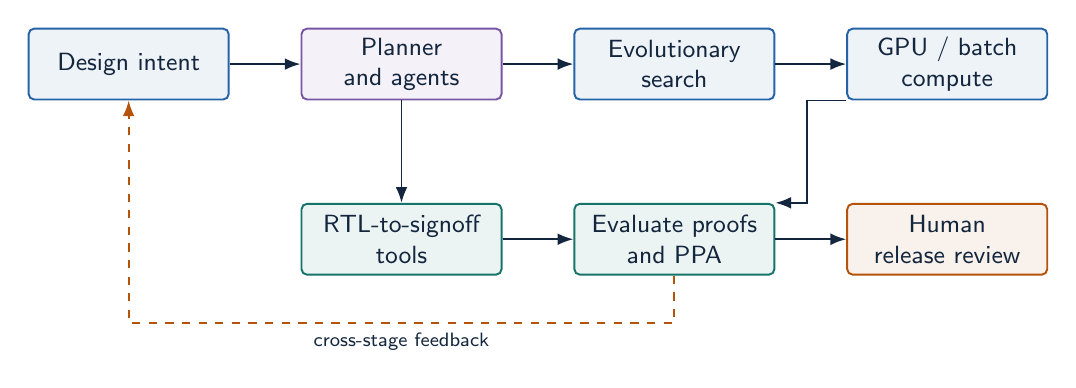
\begin{tikzpicture}[node distance=13mm and 9mm]
  \node[front] (intent) {Design intent};
  \node[verify, right=of intent] (plan) {Planner and agents};
  \node[front, right=of plan] (search) {Evolutionary search};
  \node[front, right=of search] (gpu) {GPU / batch compute};
  \node[physical, below=of plan] (tools) {RTL-to-signoff\\tools};
  \node[physical, below=of search] (eval) {Evaluate proofs and PPA};
  \node[release, below=of gpu] (release) {Human\\release review};

  \foreach \from/\to in {intent/plan,plan/search,search/gpu,plan/tools,tools/eval,eval/release}
    \draw[edaflow] (\from) -- (\to);
  \draw[edaflow] (gpu.south west) -- ++(-5mm,0) |- (eval.north east);
  \draw[edafeedback] (eval.south) -- ++(0,-6mm)
    -| node[pos=.25,below,edalabel] {cross-stage feedback} (intent.south);
\end{tikzpicture}
\end{document}
